\section{Conceptual Design}

This section describes the initial stage of the two aircraft design. The goal is to identify the optimal configuration that would provide the highest mission score.


%%%%%%%%%%%%%%%%%%%%%%%%%%%%%%%%%%%%%%%%%%%%%%%%%%%%%%%%%%%%%%%%%%%%%%%%%%%%%%%%%%%%%%
%%%%%%%%%%%%%%%%%%%%%%%%%  			DESIGN CONSTRAINS		 %%%%%%%%%%%%%%%%%%%%%%%%%
%%%%%%%%%%%%%%%%%%%%%%%%%%%%%%%%%%%%%%%%%%%%%%%%%%%%%%%%%%%%%%%%%%%%%%%%%%%%%%%%%%%%%%

\subsection{Design Constraints}

From the design requirements, following main design constraints have been identified:

\begin{enumerate}
    \item There is no limit on a battery mass, however only NiCad or NiMH batteries are allowed
    \item Both aircraft have to be able to takeoff within \SI{100}{ft} (\SI{30.48}{m})
    \item Both aircraft should be able to land safely without taking significant damage
    \item The two aircraft must be capable of performing all missions
    \begin{enumerate}
        \item The Manufacturing Support Aircraft must be able to fly without payload
        \item The Manufacturing Support Aircraft must be able to internally carry the Production Aircraft as one or more parts
        \item The Production Aircraft must be able to internally carry a 32 oz Gatorade bottle
        
    \end{enumerate}
    \item Both aircraft should withstand wingtip test when fully loaded
    \
\end{enumerate}


[AIRFIELD SCHEME HERE FROM LAST REPORT]







%%%%%%%%%%%%%%%%%%%%%%%%%%%%%%%%%%%%%%%%%%%%%%%%%%%%%%%%%%%%%%%%%%%%%%%%%%%%%%%%%%%%%%
%%%%%%%%%%%%%%%%%%%%%%%%%  			SCORING OUTLINE			 %%%%%%%%%%%%%%%%%%%%%%%%%
%%%%%%%%%%%%%%%%%%%%%%%%%%%%%%%%%%%%%%%%%%%%%%%%%%%%%%%%%%%%%%%%%%%%%%%%%%%%%%%%%%%%%%
\subsection{Scoring Outline} \label{sec:scoring_outline}
In order to understand the sensitivities of the score, the scoring formulae and the missions associated with them need to be studied. The total team score is given by

\begin{equation}
\text{Total Score} = \frac{\text{Written Report Score} \times \text{Total Mission Score}}{\text{RAC}}
\end{equation}

where \textit{RAC} is the Rated Aircraft Cost. 
%%%%%%%%%%
%%%%%%%%%%
\subsubsection{Rated Aircraft Cost}
%
Reducing $RAC$ is one of the means of achieving a higher score, as it divides the product of Report Score and Total Mission score. RAC can be calculated using the formula
%
\begin{equation}
    \text{RAC} = \text{EW}_{1} \times \text{Wt}_{\textrm{Battery 1}} \times \text{N}_{\text{comp}} + \text{EW}_{2} \times \text{Wt}_{\textrm{Battery 2}}
\end{equation}
%
where $\text{EW}_{1}$ is weight of the PA ready to fly but without payload, $\text{Wt}_{\textrm{Battery 1}}$ is battery weight for PA, $\text{N}_{\text{comp}}$ is number of sub-assemblies the PA is broken into for the delivery flight(s), $\text{EW}_{2}$ is weight of MSA ready to fly but without a payload and $\text{Wt}_{\textrm{Battery 2}}$ is battery weight for MSA

%%%%%%%%%%
%%%%%%%%%%
\subsubsection{Total Mission Score}

Total mission score is given by
%
\begin{gather}
    \textrm{Total Mission Score} = \text{MF}_{1} \times \text{MF}_{2} \times \text{PF} + \textrm{Bonus}
\end{gather}
%
where $\text{MF}_{1}$ and $\text{MF}_{2}$ are scores for the MSA flight missions, $\text{PF}$ is score for PA flight mission and $\textrm{Bonus}$ is bonus task score for PA ground mission. All flight missions require takeoff within the prescribed field length and a successful landing(s). The components of total mission score are as follows

\paragraph{MSA Arrival Flight, $\text{MF}_{1}$}

The first mission requires MSA to takeoff, fly 3 laps without a payload around the competition course within 5 minutes and land. The score from the mission is $\text{MF}_{1} = 2.0$ if the mission is completed else the score is $\text{MF}_{1} = 0.1$. The competition course layout is shown in Figure \ref{fig:course}.
%
\begin{figure}[h]
    \centering
    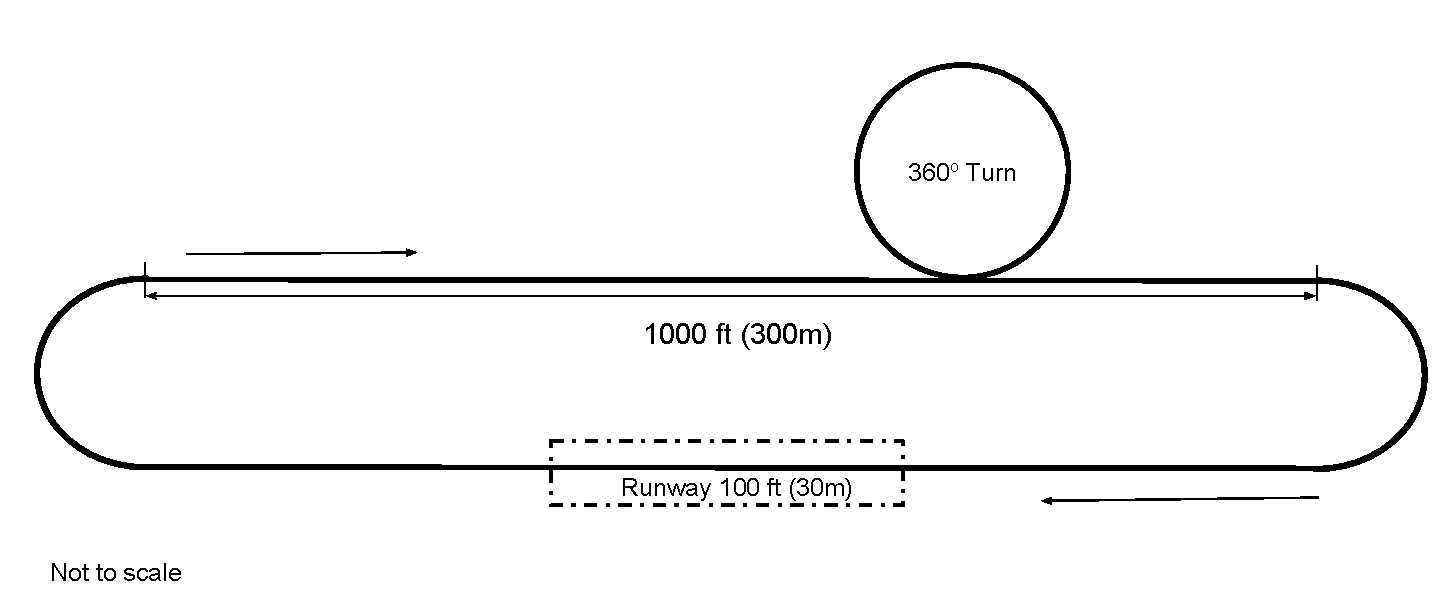
\includegraphics[width=0.8\textwidth]{course.pdf}
    \caption{Layout of the competition course}
    \label{fig:course}
\end{figure}
%

\paragraph{MSA Delivery Flight, $\text{MF}_{2}$}

The second mission requires MSA to carry PA sub-assemblies around the course. One or more parts of PA can be carried in a single flight. The MSA has to takeoff, fly one lap and land for each sub-assembly delivery flight. After landing MSA has to taxi to a payload loading area where the installed sub-assembly is removed and new sub-assembly is loaded if required. This is repeated until all PA sub-assemblies have been delivered. All PA parts need to be carried internally and the mission has to be completed within 10 minutes. The score for the mission is $\text{MF}_{2} = 4.0$ if all sub-assembly delivery flights are successfully completed, $\text{MF}_{2} = 1.0$ if at least one sub-assembly group is successfully delivered and $\text{MF}_{2} = 0.1$ if none of the above. If a partial score is received ($\text{MF}_{2} = 1.0$), the aircraft can attempt a single retry of the mission. 

\paragraph{PA Flight, $\text{PF}$}

Third mission uses PA to fly a single \SI{32}{oz} \textit{Gatorade} bottle of any flavour 3 laps around the course within 5 minutes. The payload must be carried internally. Approximate specifications of the payload are: height \SI{8.2}{in} (\SI{20.8}{\centi\meter}), maximum diameter \SI{3.7}{in} (\SI{9.4}{\centi\meter}) and mass \SI{2}{lb} \SI{3.9}{oz} (\SI{1020}{\gram}). The payload can be seen in Figure \ref{fig:gatorade}.
%
\begin{figure}[h]
    \centering
    
\includegraphics[angle=270, width=0.5\textwidth]{gatorade.jpg}
    \caption{\SI{32}{oz} \textit{Gatorade} bottle used as the payload for mission 3}
    \label{fig:gatorade}
\end{figure}
%
A score of $\text{PF} = 2.0$ will be awarded for completing all mission objectives. If PA flies less than the required number of laps or exceeds the time limit, $\text{PF} = 1.0$ is awarded. In case of no flight attempt or a complete successful flight, $\text{PF} = 0.1$ is used.  If a partial score is received ($\text{PF} = 1.0$), the aircraft can attempt a single retry of the mission. 

\paragraph{Bonus Mission}

Bonus mission requires the team to assemble PA from its sub-assemblies within 2 minutes. This includes installing and securing the payload. The mission can only be attempted if MSA successfully completed mission 2 ($\text{MF}_{2} = 4.0$). The aircraft will receive a score of $\text{Bonus} = 2.0$ if PA is assembled in the given time and passes the wing tip test and control systems check. Else $\text{Bonus} = 0.0$

%%%%%%%%%%
%%%%%%%%%%

\subsection{Total Score and Sensitivity}

From Section \ref{sec:scoring_outline}, it can be concluded that in case all mission requirements are met, the only opportunity for the score improvement lies in Written Report Score and RAC. Thus, a sensitivity analysis has been performed to asses the impact of different configurations on RAC.\\

Three different configurations have been analysed as the most viable ones: 
\begin{itemize}
    \item $\text{N}_{\text{comp}}$ = 1, 1 laps in Mission 2
    \item $\text{N}_{\text{comp}}$ = 2, 2 laps in Mission 2
    \item $\text{N}_{\text{comp}}$ = 2, 1 lap in Mission 2
\end{itemize}

3 components option was also considered for different numbers of laps in Mission 2, however it would always produce higher RAC, since with $\text{N}_{\text{comp}} = 3$,  $\text{EW}_{1} \times \text{Wt}_{\textrm{Battery 1}} \times \text{N}_{\text{comp}}$ outweighs any benefit obtained by reducing $\text{EW}_{2} \times \text{Wt}_{\textrm{Battery 2}}$.\\

First analysed 1 flight 1 component vs 2 flight 2 components!\\


The analysis was primarily based on the ratio of $m_{{ac}}$ to $m_{payload}$ and $m_{{ac}}$ to $m_{battery}$. Those ratios were defined separately for 3 different configurations and were determined to be the main variables defining the RAC. The ratios were initially taken based on team's previous experience as well as past competition reports. The initial ratios can be found in Table \ref{fig:sens_constants}. \\

\begin{figure}[!h]
    \centering
    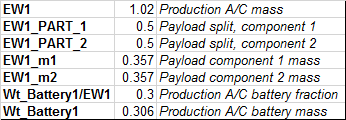
\includegraphics{sens_constants}
    \caption{Experienced based initial conditions \_PLACEHOLDER }
    \label{fig:sens_constants}
\end{figure}

Part below is analysis of 1 flight N=2 vs 2 flight N=2.\\

The aircraft carrying 2 components at the same time would have to carry a higher payload than the aircraft making 2 flights and carrying 1 component at a time. If the design is well optimised, it would mean that the former would require a heavier structure than the latter. Also, carrying more structural mass and having to take off with a higher payload, it would require more power for takeoff, and hence the propulsion mass would be higher as well. On the other hand, splitting the Production aircraft with chosen configuration to two components means that in terms of external dimensions, practically identical fuselage is required to carry either 1 component or 2 components. This means that 1 lap 2 components Manufacturing Aircraft configuration is likely to be more volume efficient, and thus it should be possible to achieve a better payload ratio. For that reason, it was always assumed that 2 components, 1 lap option Manufacturing Support Aircraft will have a lower mass of aircraft to mass of payload ratio.\\

Since Mission 1 requires the Manufacturing Aircraft to be able to fly 3 laps, it was first assumed that meeting this requirement would automatically allow flying 2 laps tp carry 2 components in Mission 2. The later concern was, however, that NiMH cells are known to produce less power after some discharge, and there might be a requirement to have a higher capacity battery to be able to produce the required power for the second takeoff in $\text{N}_{\text{comp}} = 2$, 2 laps case. For that purpose a number of the most likely ratios of $\text{EW1} / m_{payload}$ were identified. Then the RAC was calculated for a baseline case for both configuration, assuming the battery mass would be $30\%$ of the EW2. From that baseline, the battery mass fraction for 2 components, 2 flights option was changed to match the RAC of 2 components, 1 flight. This provides the headroom available for battery mass increase, as can be seen in Table \ref{fig:sens_config}.

\begin{figure}[!h]
    \centering
    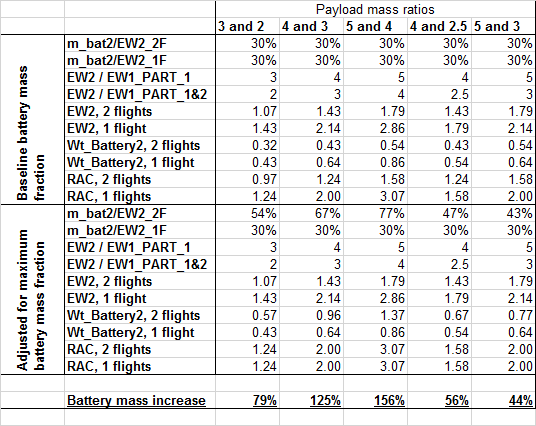
\includegraphics{sens_config}
    \caption{Number of flights for $\text{N}_{\text{comp}} = 2$ battery sensitivity analysis \_PLACEHOLDER }
    \label{fig:sens_config}
\end{figure}



As can be seen, there is plenty of battery mass penalty headroom for even the most conservative payload ratios, which implies that 2 components, 2 laps option will allow getting the highest RAC and thus the highest score possible.

how to determine number of components and flights\\



briefly intro 3 comnp 3 flights\\


%%%%%%%%%%%%%%%%%%%%%%%%%%%%%%%%%%%%%%%%%%%%%%%%%%%%%%%%%%%%%%%%%%%%%%%%%%%%%%%%%%%%%%
%%%%%%%%%%%%%%%%%%%%%%%%%  		CONFIGURATION SELECTION		 %%%%%%%%%%%%%%%%%%%%%%%%%
%%%%%%%%%%%%%%%%%%%%%%%%%%%%%%%%%%%%%%%%%%%%%%%%%%%%%%%%%%%%%%%%%%%%%%%%%%%%%%%%%%%%%%

\subsection{Configuration Selection}

%%%%%%%%%%
%%%%%%%%%%

Mission 3 requires PA to carry the specified payload internally. Thus the team decided to design the fuselage to follow the shape of the payload as closely as possible to reduce the dimensions and the mass of the aircraft. On the other hand, the main purpose of MSA is to carry the sub-assemblies of PA internally around the competition course in mission 2. Thus the driving factor in fuselage selection for MSA is to fit the PA sub-assemblies into MSA with minimum structural requirements.

From sensitivity analysis, it was concluded that two flights in mission 2, carrying PA in two separate sub-assemblies would provide the highest score. Therefore to minimise the mass of MSA, the two PA sub-assemblies should be of similar mass and dimensions. This approach avoids wasting internal volume of MSA and makes sure that MSA payload requirement is as low as possible. The heavier piece would be carried first to take advantage of a fresh battery pack and make the second takeoff with partially discharged batteries less demanding.

Flying wing configuration was initially considered since it would provide efficient use of volume when one flying wing is place inside another one. However the advantage over a conventional design was analysed to be far less if the aircraft can be split into two components because the wing/landing gear group and the fuselage/boom/tail group can be with relative ease designed to provide two slender bodies with similar dimensions and masses. Also conventional design was judged to be a less risky option.

Therefore for PA, the wing span should closely align with the overall length of the aircraft and the wing chord and landing gear height should be close to the diameter of the PA fuselage. Furthermore the horizontal and vertical tail should not reach much outside the diameter of the fuselage. The approach chosen drove the team to adopt a tail dragger landing gear since this would eliminate the need for a relatively large front landing gear. However the team was unable to locate the vertical tail upside down compared to a regular configuration due to roll angle requirements. Thus the 